%%%%%%%%%%%%%%%%%%%%%%%%%%%%%%%%%%%%%%%%%
% Structured General Purpose Assignment
% LaTeX Template
%
% This template has been downloaded from:
% http://www.latextemplates.com
%
% Original author:
% Ted Pavlic (http://www.tedpavlic.com)
%
% Note:
% The \lipsum[#] commands throughout this template generate dummy text
% to fill the template out. These commands should all be removed when 
% writing assignment content.
%
%%%%%%%%%%%%%%%%%%%%%%%%%%%%%%%%%%%%%%%%%

%----------------------------------------------------------------------------------------
%	PACKAGES AND OTHER DOCUMENT CONFIGURATIONS
%----------------------------------------------------------------------------------------

\documentclass{article}

\usepackage{fancyhdr} % Required for custom headers
\usepackage{lastpage} % Required to determine the last page for the footer
\usepackage{extramarks} % Required for headers and footers
\usepackage{graphicx} % Required to insert images
\usepackage{listings} % code listings
\usepackage{cprotect}
\usepackage{xifthen}
\usepackage{tabularx}
\usepackage{multirow}
\usepackage{color}
\usepackage{datetime}
\usepackage[normalem]{ulem}

% Margins
\topmargin=-0.45in
\evensidemargin=0in
\oddsidemargin=0in
\textwidth=6.5in
\textheight=9.0in
\headsep=0.25in 

\linespread{1.1} % Line spacing

% Colors
\definecolor{stringcolor}{rgb}{0.58,0,0.82}
\definecolor{kwordcolor}{rgb}{0,0,1.0}
\definecolor{gray}{rgb}{0.5,0.5,0.5}

% Listings
\lstset{basicstyle=\ttfamily}
\lstset{
    language=C,
    basicstyle=\small\ttfamily,
    keywordstyle=\color{kwordcolor},
    stringstyle=\color{stringcolor},
    frame=single,
    numbers=left,
    stepnumber=1,
    numberstyle=\small\color{gray},
    numbersep=10pt,
    morekeywords={uint64_t, uint32_t, uint16_t, uint8_t,
                  int64_t,  int32_t,  int16_t,  int8_t}
}


% Set up the header and footer
\pagestyle{fancy}
\lhead{\hmwkAuthorName} % Top left header
\chead{\hmwkClass: \hmwkTitle} % Top center header
\rhead{\firstxmark} % Top right header
\lfoot{\lastxmark} % Bottom left footer
\cfoot{} % Bottom center footer
\rfoot{Page\ \thepage\ of\ \pageref{LastPage}} % Bottom right footer
\renewcommand\headrulewidth{0.4pt} % Size of the header rule
\renewcommand\footrulewidth{0.4pt} % Size of the footer rule

\setlength\parindent{0pt} % Removes all indentation from paragraphs

%----------------------------------------------------------------------------------------
%	DOCUMENT STRUCTURE COMMANDS
%	Skip this unless you know what you're doing
%----------------------------------------------------------------------------------------

% Header and footer for when a page split occurs within a problem environment
\newcommand{\enterProblemHeader}[1]{
\nobreak\extramarks{#1}{#1 continued on next page\ldots}\nobreak
\nobreak\extramarks{#1 (continued)}{#1 continued on next page\ldots}\nobreak
}

% Header and footer for when a page split occurs between problem environments
\newcommand{\exitProblemHeader}[1]{
\nobreak\extramarks{#1 (continued)}{#1 continued on next page\ldots}\nobreak
\nobreak\extramarks{#1}{}\nobreak
}

\setcounter{secnumdepth}{0} % Removes default section numbers
\newcounter{homeworkProblemCounter} % Creates a counter to keep track of the number of problems

\newcommand{\homeworkProblemName}{}
\newenvironment{homeworkProblem}[1][Problem \arabic{homeworkProblemCounter}]{ % Makes a new environment called homeworkProblem which takes 1 argument (custom name) but the default is "Problem #"
\stepcounter{homeworkProblemCounter} % Increase counter for number of problems
\renewcommand{\homeworkProblemName}{#1} % Assign \homeworkProblemName the name of the problem
\section{\homeworkProblemName} % Make a section in the document with the custom problem count
\enterProblemHeader{\homeworkProblemName} % Header and footer within the environment
}{
\exitProblemHeader{\homeworkProblemName} % Header and footer after the environment
}

\newcommand{\problemAnswer}[2][]{ % Defines the problem answer command with the content as the only argument
\noindent\framebox[\columnwidth][c]{
\begin{minipage}{0.98\columnwidth}
#2

\ifthenelse{\isempty{#1}}{}{\textbf{Answer: #1.}}
\end{minipage}
} % Makes the box around the problem answer and puts the content inside, with an optional bolded answer
}

\newcommand{\homeworkSectionName}{}
\newenvironment{homeworkSection}[1]{ % New environment for sections within homework problems, takes 1 argument - the name of the section
\renewcommand{\homeworkSectionName}{#1} % Assign \homeworkSectionName to the name of the section from the environment argument
\subsection{\homeworkSectionName} % Make a subsection with the custom name of the subsection
\enterProblemHeader{\homeworkProblemName\ [\homeworkSectionName]} % Header and footer within the environment
}{
\enterProblemHeader{\homeworkProblemName} % Header and footer after the environment
}
   
%----------------------------------------------------------------------------------------
%	NAME AND CLASS SECTION
%----------------------------------------------------------------------------------------

\newcommand{\hmwkTitle}{Project Report} % Assignment title
\newcommand{\hmwkDueDate}{\formatdate{29}{4}{2016}} % Due date
\newcommand{\hmwkClass}{ECEN\ 4593} % Course/class
\newcommand{\hmwkAuthorName}{Brook Hernandez and Austin Glaser} % Your name
\newcommand{\hmwkAuthorNumber}{101-08-7347 and 810-92-4163} % Student Number

%----------------------------------------------------------------------------------------
%	TITLE PAGE
%----------------------------------------------------------------------------------------

\title{
\vspace{2in}
\textmd{\textbf{\hmwkClass:\ \hmwkTitle}}\\
\normalsize\vspace{0.1in}\small{Due\ on\ \hmwkDueDate}\\
\vspace{3in}
}

\author{
\textbf{\hmwkAuthorName} \\
\hmwkAuthorNumber
}
\date{\today} % Insert date here if you want it to appear below your name

%----------------------------------------------------------------------------------------

\begin{document}

\maketitle

%----------------------------------------------------------------------------------------
%	TABLE OF CONTENTS
%----------------------------------------------------------------------------------------

%\setcounter{tocdepth}{1} % Uncomment this line if you don't want subsections listed in the ToC

%\newpage
%\tableofcontents
\newpage

%----------------------------------------------------------------------------------------
%	Introduction
%----------------------------------------------------------------------------------------

\section{Introduction}

The goal of the Memory Simulation project was to implement a simulator that can simulate and evaluate a memory system with two levels of cache memory and a main memory. Within the system there is a level-1 (L1) instruction cache and a L1 data cache. There is also a unified level-2 (L2) cache which handles requests from both L1 caches. Misses that occur in the L2 cache are handled by main memory. These caches are write-allocate, write-back caches with an 8-entry victim cache. 

\section{Simulation Results}

\section{Trend Analysis}

\subsection{Miss Rate and Cache Size Analysis}

Comparing the miss rates and the cache sizes, we can see in figure \ref{fig:L1imissvsl1isize}, \ref{fig:l1vsmiss}, and \ref{fig:l2vsmiss} that as the cache size increases, the miss rates for the most part decrease. We expected this in most cases because as the cache size increases there is less chance of a conflict. It can be see in figure \ref{fig:l2vsmiss} that there is an exception to our expected results. The miss rate for the bzip2 trace increases slightly as the cache size increases. This could be because...

\section{Main Memory System Analysis}

One major task in this project was to determine the effect the bandwidth of the
main memory connection has on memory system performance. We only performed the
simulations on the `sjeng` trace, so the plots have less data. Before examining
the results of the simulations, we can make a couple of predictions based around
our knowledge of the memory system's functionality.

The first is that, all other configuration details being equal, there will be no
performance improvement with a bus width greater than 64 bytes. The fastest main
memory access possible will need to transfer a single block of data to or from
the L2 cache, and since that transfer will always be 64 bytes of data, larger
busses will simply be wasted bandwidth.

Secondly, we can expect diminishing returns with each doubling in bandwidth.
There is a constant-time aspect to the memory access (sending the address and
waiting for the memory to be ready), and we're making no changes to that aspect
of the system. As long as this is the case (according to our friend Amdahl),
there is a performance limit which is insurmountable even if we could spend zero
time actually transferring data. Furthermore, these constant time operations
occupy an increasing proportion of our total memory access time.

Now, on to the actual results. Examining figure \ref{fig:cpivsband} shows us
that our predictions are borne out by the actual data -- the largest performance
improvement comes from the first doubling, while later doublings produce
progressively smaller impacts.

We can also look at the relationship between cost and performance (figure
\ref{fig:cpivsmainmemcost}). This is particularly interesting, because the
performance curve flattens out somewhat, becoming somewhat closer to linear.
This means that, from a cost/benefit standpoint, greater memory bandwidths
actually start to look MORE attractive rather than less, even given the
diminishing returns outlined above.

It begins to make sense in light of the chosen cost function, which is actually
logarithmic (ignoring latency, it's $\$75 + \$100 \log_2(B / 8)$, where $B$ is
the memory bandwidth in bytes). To us, this seems slightly unrealistic---our
first instinct is that this function should be linear or worse. However, it does
explain the results, and when taken as a given makes higher-bandwidth main
memory interfaces look even more attractive.

\begin{figure}[ht]
    \centering
    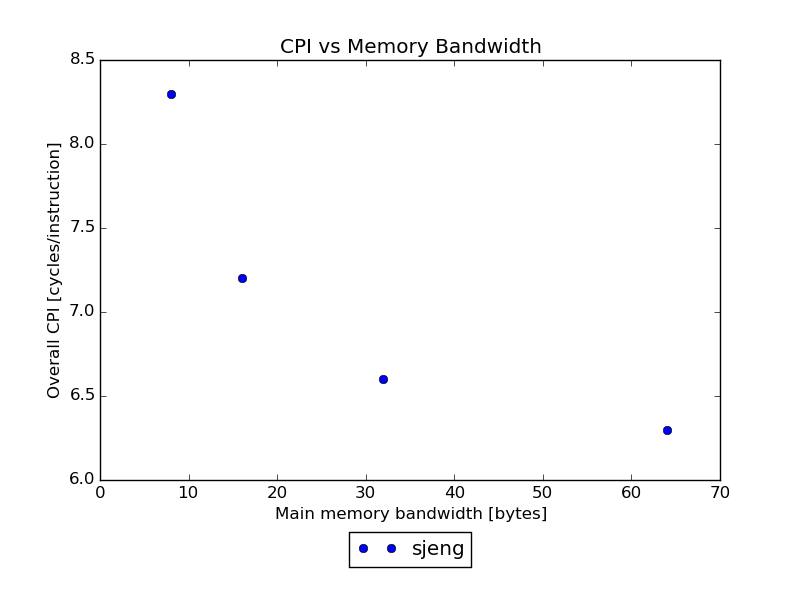
\includegraphics[width=0.75\textwidth]{plots/CPI_vs_Bandwidth.png}
    \caption{Performance impact of main memory bandwidth}
    \label{fig:cpivsband}
\end{figure}

\begin{figure}[ht]
    \centering
    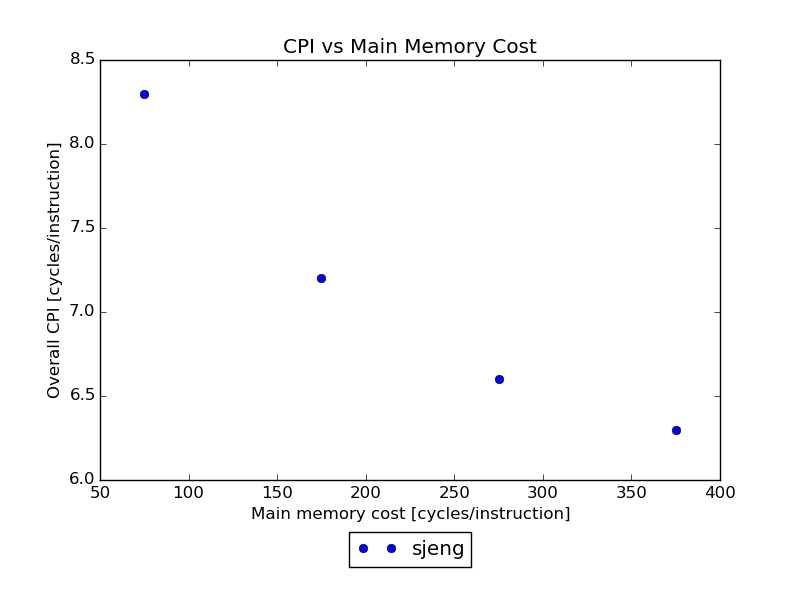
\includegraphics[width=0.75\textwidth]{plots/CPI_vs_Main_Mem_Cost.png}
    \caption{Performance impact of main memory cost}
    \label{fig:cpivsmainmemcost}
\end{figure}

\begin{figure}[ht]
    \centering
    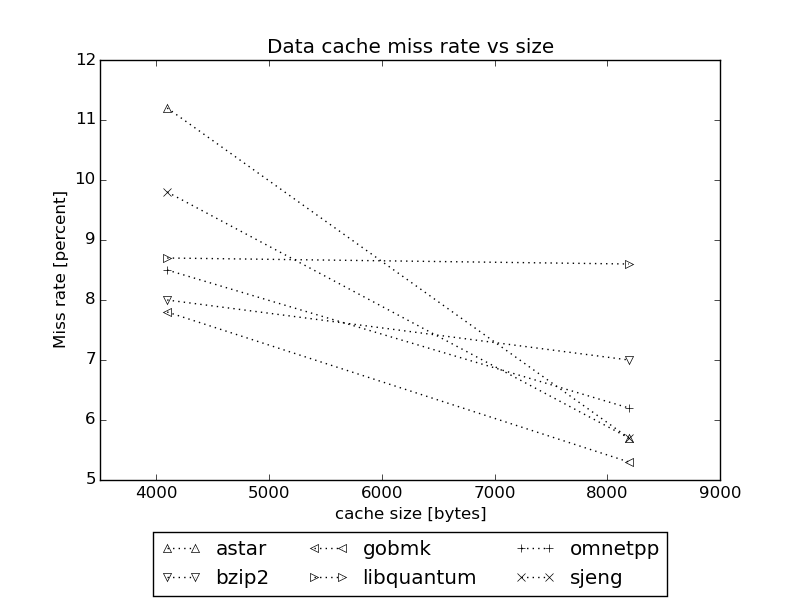
\includegraphics[width=0.75\textwidth]{plots/L1_Dcache_miss_vs_L1_Dcache_size.png}
    \caption{Size of L1 Dcache impact on L1 Dcache miss rate}
    \label{fig:l1vsmiss}
\end{figure}

\begin{figure}[ht]
    \centering
    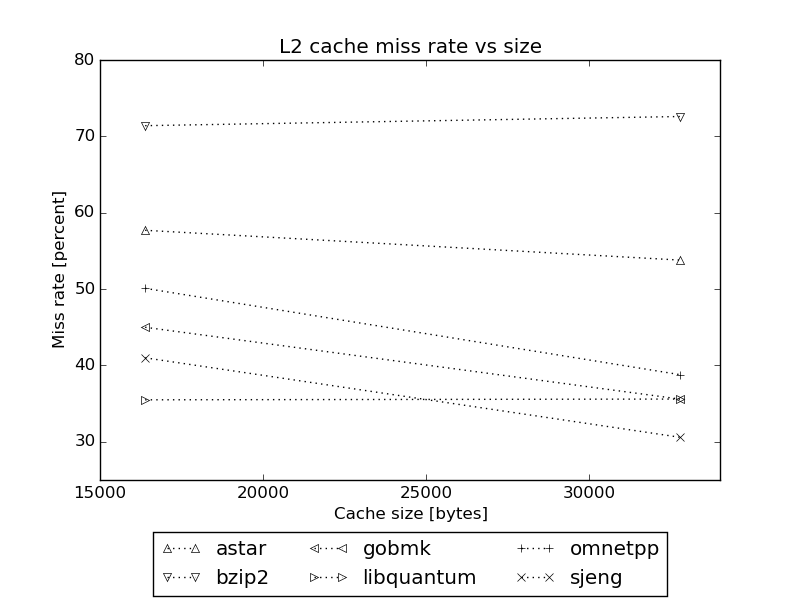
\includegraphics[width=0.75\textwidth]{plots/L2cache_miss_vs_size.png}
    \caption{Size of L2 cache impact on L2 cache miss rate}
    \label{fig:l2vsmiss}
\end{figure}

\begin{figure}[ht]
    \centering
    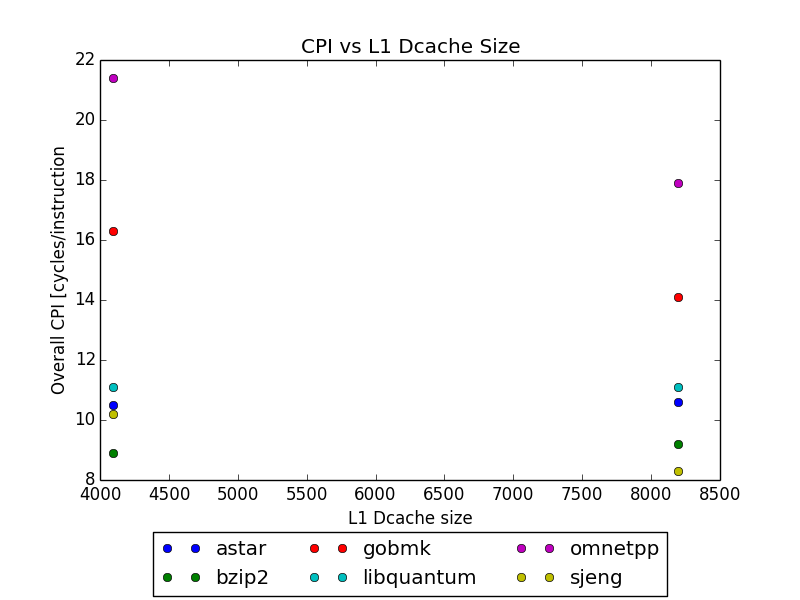
\includegraphics[width=0.75\textwidth]{plots/CPI_vs_L1Dcache_size.png}
    \caption{Performance impact with L1 Dcache size}
    \label{fig:cpivsl1size}
\end{figure}

\begin{figure}[ht]
    \centering
    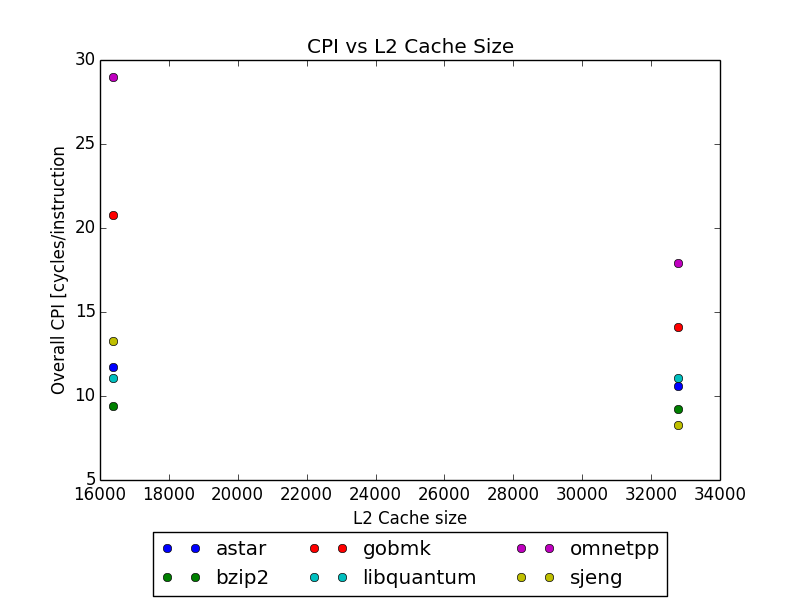
\includegraphics[width=0.75\textwidth]{plots/CPI_vs_L2Cache_size.png}
    \caption{Performance impact with L2 Cache size}
    \label{fig:cpivsl2size}
\end{figure}

\begin{figure}[ht]
    \centering
    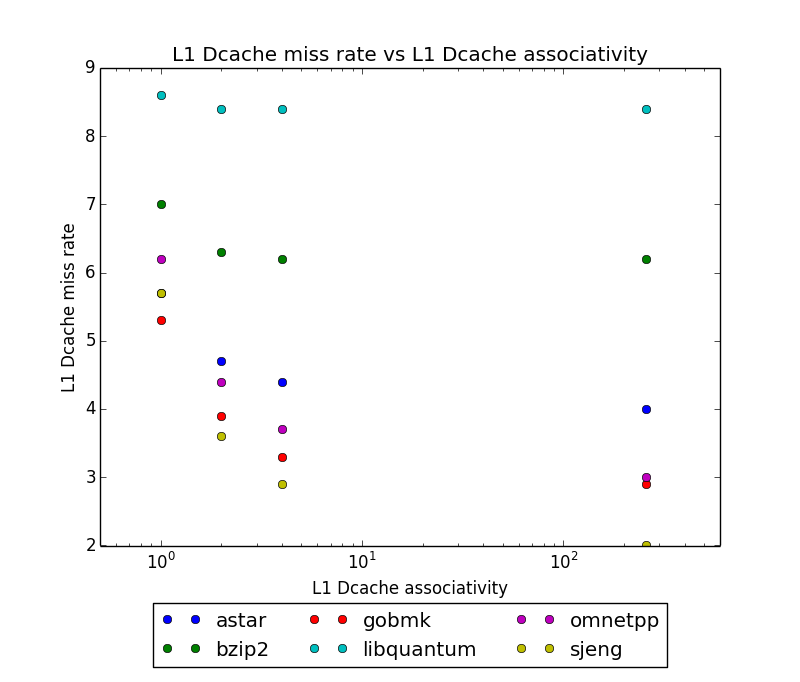
\includegraphics[width=0.75\textwidth]{plots/L1Dcache_miss_vs_associativity.png}
    \caption{L1 Dcache miss rate vs L1 Dcache Associativity}
    \label{fig:l1missvsl1assoc}
\end{figure}

\begin{figure}[ht]
    \centering
    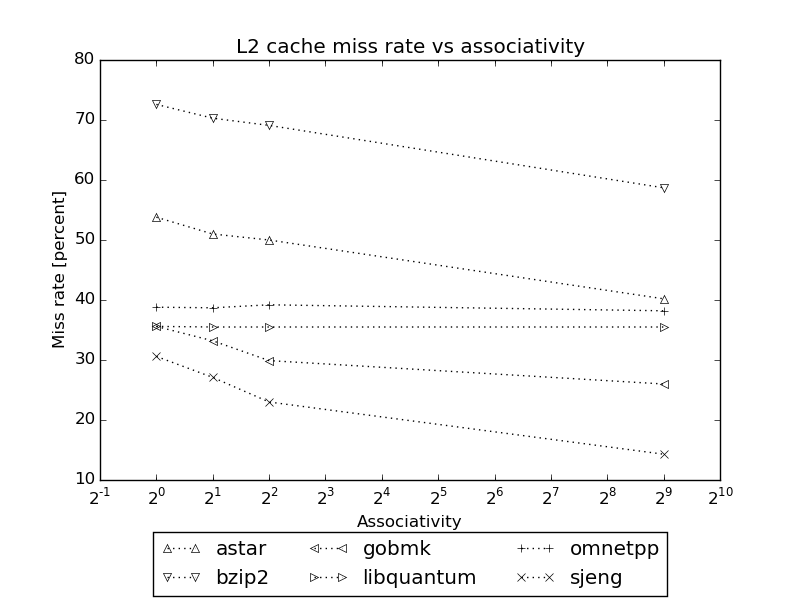
\includegraphics[width=0.75\textwidth]{plots/L2cache_miss_vs_L2cache_associativity.png}
    \caption{L2 cache miss rate vs L2 cache Associativity}
    \label{fig:l2missvsl2assoc}
\end{figure}

\begin{figure}[ht]
    \centering
    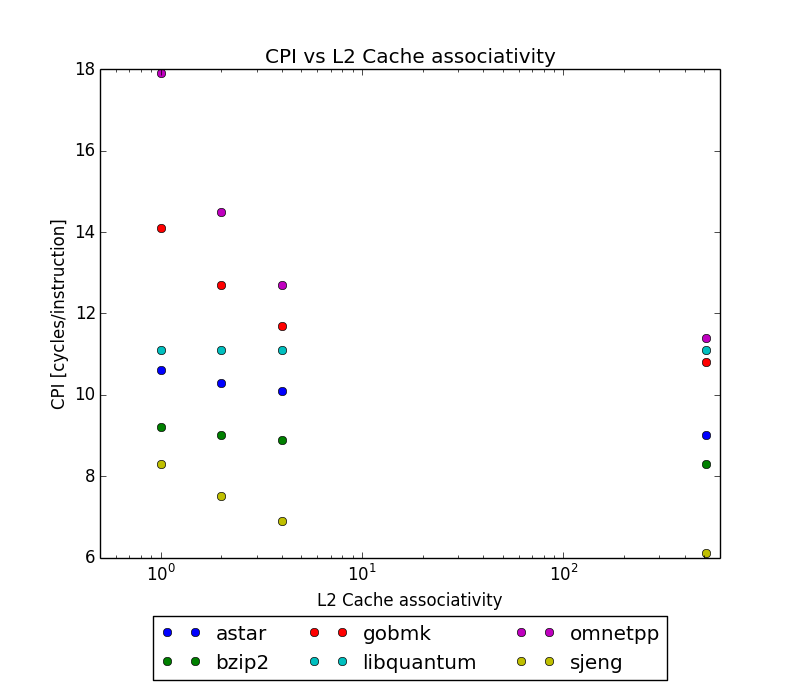
\includegraphics[width=0.75\textwidth]{plots/CPI_vs_L2Cache_associativity.png}
    \caption{Performance impact on L2 cache associativity}
    \label{fig:cpivsl2assoc}
\end{figure}

\begin{figure}[ht]
    \centering
    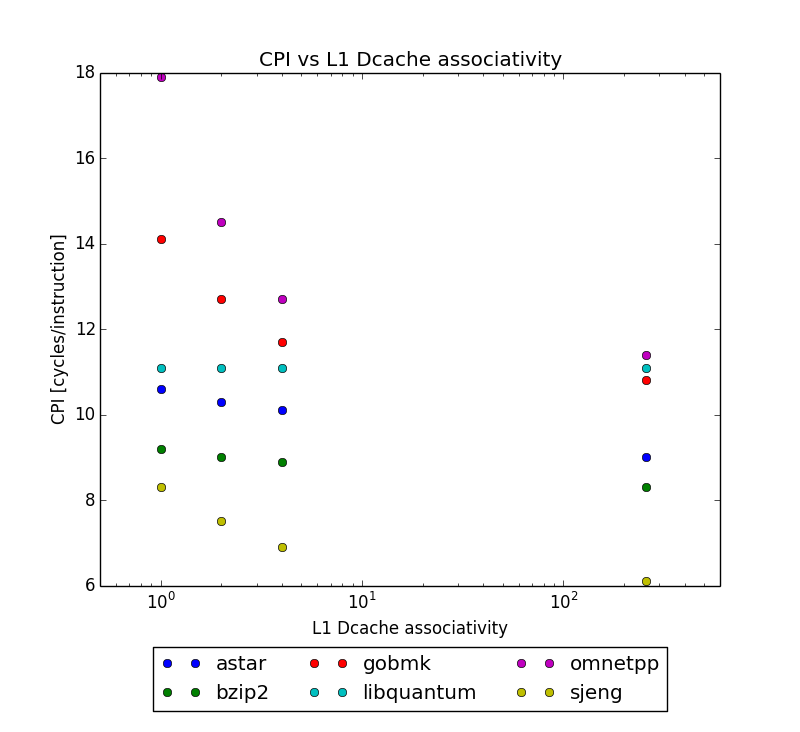
\includegraphics[width=0.75\textwidth]{plots/CPI_vs_L1Dcache_associativity.png}
    \caption{Performance impact on L1 Dcache associativity}
    \label{fig:cpivsl1assoc}
\end{figure}

\begin{figure}[ht]
    \centering
    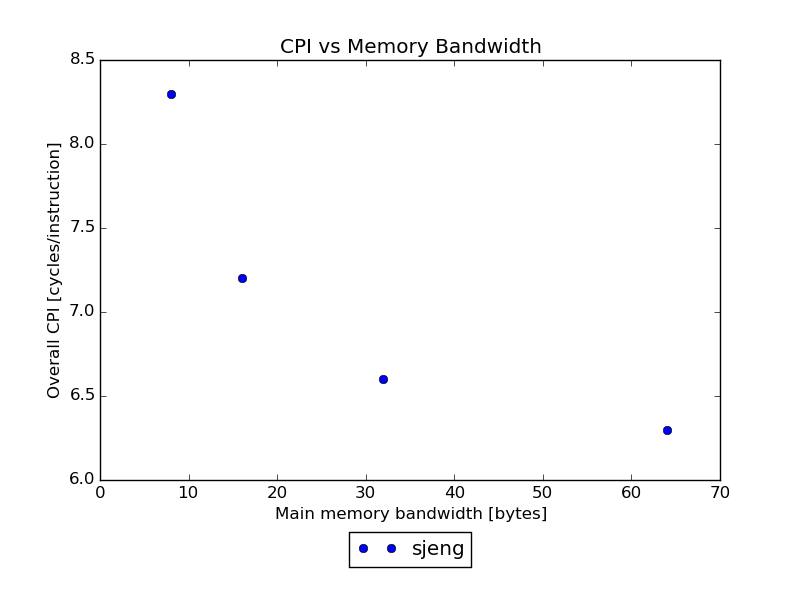
\includegraphics[width=0.75\textwidth]{plots/CPI_vs_Bandwidth.png}
    \caption{Performance impact vs Main Memory Bandwidth}
    \label{fig:cpivsbandwidth}
\end{figure}

\begin{figure}[ht]
    \centering
    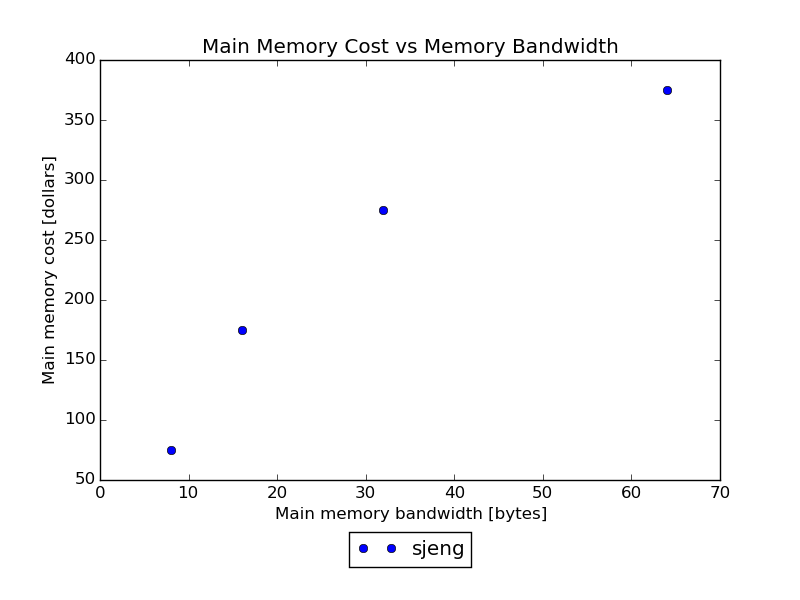
\includegraphics[width=0.75\textwidth]{plots/Cost_vs_Bandwidth.png}
    \caption{Main memory cost vs Main Memory Bandwidth}
    \label{fig:costvsbandwidth}
\end{figure}

\begin{figure}[ht]
    \centering
    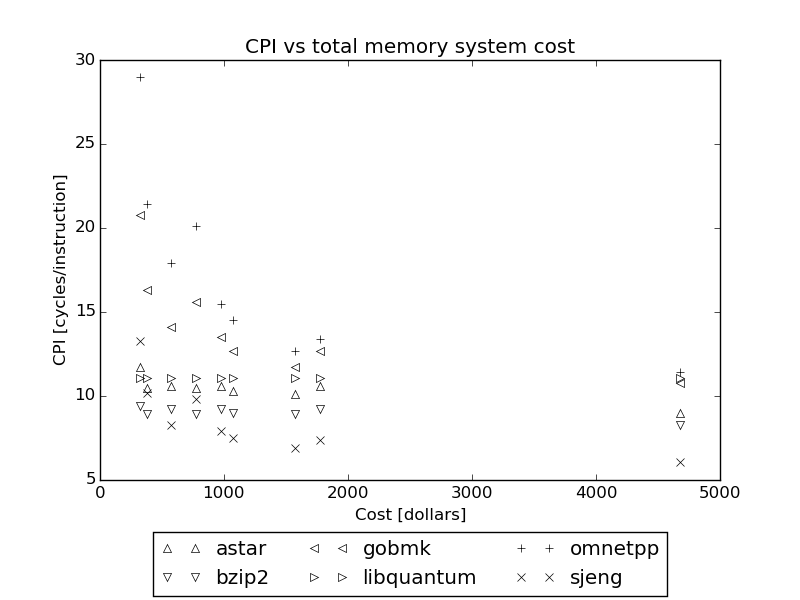
\includegraphics[width=0.75\textwidth]{plots/CPI_vs_Total_memory_system_cost.png}
    \caption{Performance vs Total main memory cost}
    \label{fig:cpivstotalcost}
\end{figure}

\begin{figure}[ht]
    \centering
    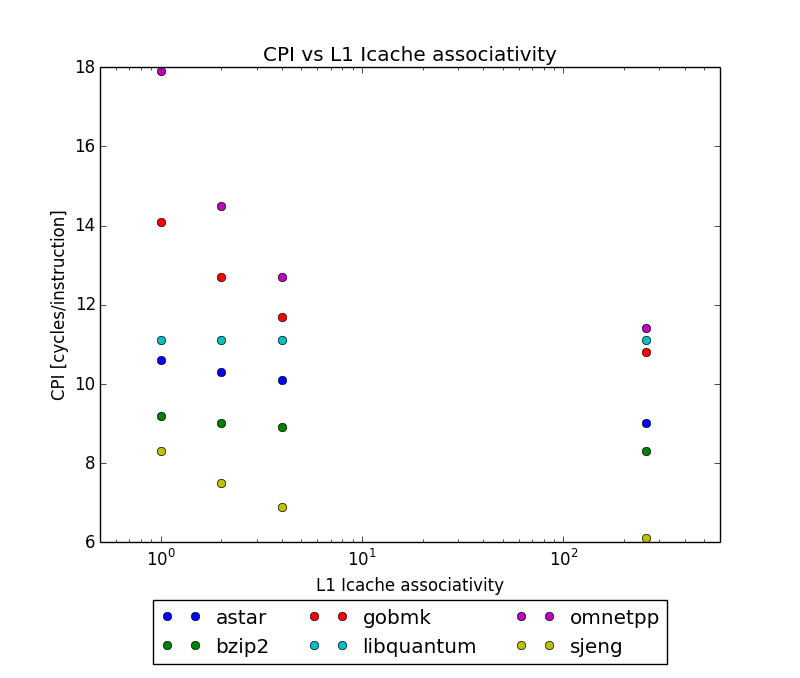
\includegraphics[width=0.75\textwidth]{plots/CPI_vs_L1icache_assoc.png}
    \caption{Performance vs L1 Icache Associativity}
    \label{fig:cpivsl1iassoc}
\end{figure}

\begin{figure}[ht]
    \centering
    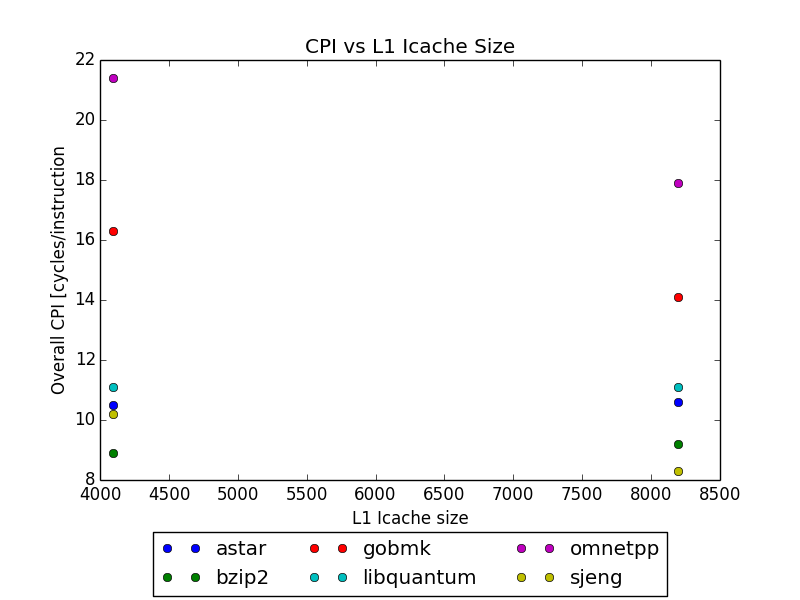
\includegraphics[width=0.75\textwidth]{plots/CPI_vs_L1icache_size.png}
    \caption{Performance vs L1 Icache Size}
    \label{fig:cpivsl1isize}
\end{figure}

\begin{figure}[ht]
    \centering
    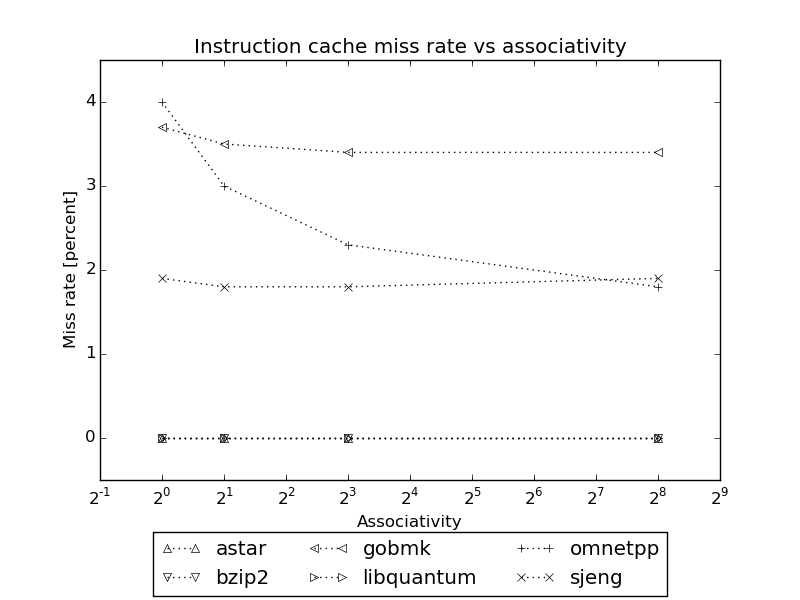
\includegraphics[width=0.75\textwidth]{plots/L1icache_miss_vs_L1icache_Assoc.png}
    \caption{L1 Icache Miss Rate vs L1 Icache Associativity}
    \label{fig:L1imissvsl1iassoc}
\end{figure}

\begin{figure}[ht]
    \centering
    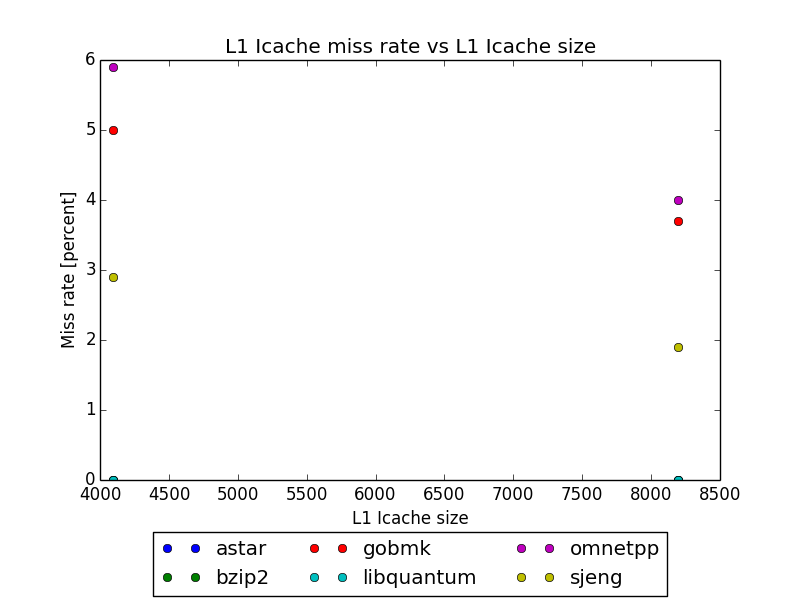
\includegraphics[width=0.75\textwidth]{plots/L1icache_miss_vs_L1icache_size.png}
    \caption{L1 Icache Miss Rate vs L1 Icache Size}
    \label{fig:L1imissvsl1isize}
\end{figure}


\clearpage
\appendix
\section{Source Code}

This section contains the raw source code for the simulator. It omits test
suites, though this simulator does have a full suite of accompanying unit tests.
(they exist at under the \texttt{test/} directory at the top-level).

Files are broken by type, and then alphabetically

\subsection{Header Files}

\lstinputlisting[caption=Memory access utilities interface, label=lst:access_h]{../../inc/Access.h}
\clearpage
\lstinputlisting[caption=Cache data management interface, label=lst:cachedata_h]{../../inc/CacheData.h}
\clearpage
\lstinputlisting[caption=Cache cycles and interaction interface, label=lst:cacheinternals_h]{../../inc/CacheInternals.h}
\clearpage
\lstinputlisting[caption=Third-party exception library configuration, label=lst:cexceptionconfig_h]{../../inc/CExceptionConfig.h}
\clearpage
\lstinputlisting[caption=Configuration management interface, label=lst:config_h]{../../inc/Config.h}
\clearpage
\lstinputlisting[caption=Definitions for exception types, label=lst:exceptiontypes_h]{../../inc/ExceptionTypes.h}
\clearpage
\lstinputlisting[caption=L1 Cache simulator interface, label=lst:l1cache_h]{../../inc/L1Cache.h}
\clearpage
\lstinputlisting[caption=L2 Cache simulator interface, label=lst:l2cache_h]{../../inc/L2Cache.h}
\clearpage
\lstinputlisting[caption=Main Memory simulator interface, label=lst:mainmem_h]{../../inc/MainMem.h}
\clearpage
\lstinputlisting[caption=Simulator statistics collection interface, label=lst:statistics_h]{../../inc/Statistics.h}
\clearpage
\lstinputlisting[caption=Common utility functions interface, label=lst:util_h]{../../inc/Util.h}
\clearpage

%----------------------------------------------------------------------------------------

\end{document}
